
\newcommand{\coauthor}[2]{{\Large \textsc{#1}} {(\texttt{#2})}

    \medskip}
\newcommand{\versiontag}[2]{Versione #1 compilata il #2}
\newcommand{\gitrevision}[1]{Git sha1: #1}


\newcommand*{\stattitle}{%
  \begingroup\thispagestyle{empty}
  %\hbox{
    \hspace*{0.16\textwidth}%
    \rule{1pt}{\textheight}%
    \hspace*{0.05\textwidth}%
    \begin{minipage}[b][\textheight][b]{0.79\textwidth}

      % Title.
      {\noindent\Huge\bfseries Elementi di computazione}

      \vspace{2\baselineskip}

      % Sub-title.
      {\large \textit{Per il laboratorio di Fisica}}

      % The glorious word cloud.
      \vspace{4\baselineskip}
      \hspace*{1cm}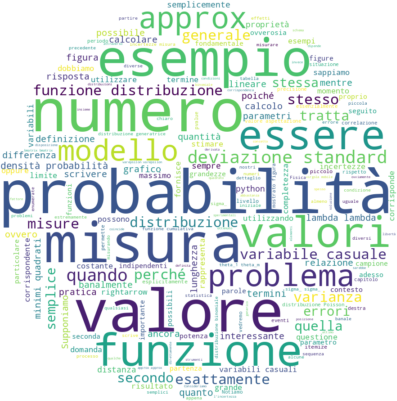
\includegraphics{figures/cover_word_cloud.png}
      \vspace{4\baselineskip}

      % Authors.
      \coauthor{Luca Baldini}{luca.baldini@pi.infn.it}
      \vspace{0.1\textheight}

      % Document version.
      \versiontag{6.2.0
}{\today}

      \smallskip

      web: \url{https://github.com/unipi-physics-labs/statnotes}

      \smallskip

      \gitrevision{\input{.git/refs/heads/main}}

      \vspace{\baselineskip}
    \end{minipage}
  %}
  \cleardoublepage
  \endgroup}
